% !TeX root = ./document.tex
\documentclass[document]{subfiles}
\begin{document}
\chapter{Метрические компакты}
Топологический компакт: из любого подпокрытия можно выбрать конечное подпокрытие.
\begin{statement}[из топологии]
    \begin{enumerate}
        \item $(X, \rho)$ -- метрическое пространство, $K \subset X$, $K$ -- компакт $\Leftrightarrow K$ -- счётно-компактен, то есть 
        \[ \forall \seq{x_n}^\infty_{n=1}, x_n \in K \quad \exists \seq{x_{n_j}}^\infty_{j=1} \text{ т.ч. } \exists \liml_{j \to \infty} x_{n_j} = x_0, \, x_0 \in K \] 
        \item $K$ -- компакт $\Rightarrow$ $K$ -- ограниченное замкнутое множество.
    \end{enumerate}
\end{statement}

\begin{example}
    $\bR^n$, $K$ -- компакт $\Leftrightarrow K$ -- ограниченное, замкнутое 
\end{example}
\begin{remark}
    НИ В КОЕМ СЛУЧАЕ!!! \\\
    $K$ -- ограниченное замкнутое, $\not \Rightarrow K$ -- компакт
\end{remark}

\begin{remark}
    $l^2 = \seq{x = \seq{x_n}^\infty_{n=1}, ||x||_2 = \left( \sum^\infty_{n=1} |x_n|^2  \right)^\frac{1}{2} < + \infty, x_n \in \bR (\bC)} $
    \[ D = \seq{ x \in l^2: ||x||_2 \leq 1} \text{ -- ограниченное, замкнутое }\] 
    $e_n = (0, 0, \ldots, 0, \underbrace{1}_n, 0, 0, \ldots),$ $n \ne m \quad ||e_n - e_m||_2 = \sqrt{2} \Rightarrow \forall \seq{e_{n_j}}$ -- не фундаментальная.
    Тогда $\nexists \, \liml_{j \to \infty} e_{n_j} \Rightarrow D$ -- не компакт.
\end{remark}


Ещё одно \textit{ напоминание}, кто такие относительно компактные множества.
\begin{definition}[относительный компакт]
    $(X, \rho), A \subset X, A$ -- относительно компактно, если $\overline{A}$ -- компакт.
    Или можно сказать 
    \[\Leftrightarrow \, \forall \seq{x_n}^\infty_{n=1}, x_n \in A \, \exists \seq{x_{n_j}}^\infty_{j=1}, \, \exists \liml_{j \to \infty} x_{n_j} = x_0, x_0 \in X \]
    Предел не обязательно принадлежит $A$.
    А в компакте предел обязательно лежит в $A$.
\end{definition}

Мы получим новое описание компактных и относительно компактных множеств. В $\bR^n$ мы описывали относительные компакты. Для описания компакта 
нужно добавить замыкание.

Еще несколько определений:
\begin{definition}[$\varepsilon$-сеть]
    $(X, \rho)$ -- метрическое пространство. $A \subset X, \varepsilon > 0$ \\
    $F$ -- $\varepsilon$-сеть для $A$, если 
    \begin{multline*}
        \forall a \in A \, \exists f \in F: \rho(a,f) < \varepsilon \\
        (\Leftrightarrow \, \forall a \in A B_\varepsilon(a) \cap F \ne \varnothing) \Leftrightarrow (A \subset \bigcup U_{f \in F} B_{\varepsilon}(f))
    \end{multline*}
\end{definition}

\begin{definition}
    $A$ -- \textbf{вполне ограниченное множество}, если для $\forall \varepsilon > 0 \, \exists$ конечная $\varepsilon$-сеть для $A$.
\end{definition}

Описание компактных и относительно-компактных множеств в терминах почти ограниченных -- как раз наша главная цель.
Мы будем использовать это новое описание так: если мы в полном метрическом пространстве, то там относительная компактность и вполне ограниченность -- одно и то же.
А проверять вполне ограниченность - гораздо проще, чем проверять относительную компактность. Предъявим $\varepsilon$-сеть и всё!

\begin{remark}
    $(X,\rho)$, $A$ -- вполне ограниченное $\Rightarrow A$ -- ограничено.
\end{remark}

\begin{example}
    $(\bR^n, || \cdot ||_2) = l^2_n \quad A \subset \bR^N$. $A$ -- ограниченное $\Leftrightarrow A$ вполне ограниченное
\end{example}

\begin{proof}
    $A$ -- ограниченное $\Leftrightarrow$ $\exists M > 0, \, \forall x - (x_1, \ldots, x_n) \in A \Rightarrow |x_j| \leq M$ \\
    $A \subset \bQ = \seq{ |x_j| \leq M, 1 \leq j \leq n}$
    Как же построить $\varepsilon$--сеть? \\ %рисунок с решеткой
    Пусть $\varepsilon > 0$, $Q = \bigcup Q_j, l$ -- cторона $Q_j$
    \begin{gather*}
        \diam Q_j = \sup_{x,y \in Q_j} \rho(x,y) = \sqrt{n} \cdot l < \varepsilon \Rightarrow l < \frac{\varepsilon}{\sqrt{n}} \\
        l = \frac{M}{N}, N \in \bN, \, \exists N: \frac{M}{N} < \frac{\varepsilon}{\sqrt{n}} \Rightarrow \\
        F \text{ -- вершины } Q_j \text{ -- } \varepsilon\text{-сеть}
    \end{gather*}
    EC = equicontinuous
    \begin{figure}
        \begin{tikzpicture}
            \pic at (0,0)   {matrix={4}{7}{}{}          {}{}};
        \end{tikzpicture}
        \caption{классный поясняющий рисуночек}
    \end{figure}
\end{proof}


Убедимся в пространстве $l^2$

\begin{example}
    $D \subset l^2, D = \seq{x \in l^2: ||x||_2 \leq 1}$
    Убедимся, что $D$ -- не вполне ограниченное.
\end{example}

\begin{proof}
    \begin{gather*}
        \seq{e_n}^\infty_{n=1}, e_n = (0, \ldots, 0, \underbrace{1}_n, 0, \ldots), n \ne m, ||e_n - e_m|| = \sqrt{2} \\
        B_{\frac{1}{2}} (e_n) \cap B_{\frac{1}{2}}(e_m) = \varnothing \\
        \varepsilon = \frac{1}{2}, F \text{ -- } \frac{1}{2}\text{-сеть для } D \\
        \Rightarrow \, \forall n \, \exists f_n \in F \cap B_{\frac{1}{2}}(e_n), \, f_n \ne f_m (n \ne m) \text{ так как } B_{\frac{1}{2}}(e_n) \cap B_{\frac{1}{2}}(e_m) = \varnothing \\
        \seq{f_n}^\infty_{n=1} \subset F \Rightarrow F \text{ -- не конечное}
    \end{gather*}
    %Базисные векторы. Пока мы не знаем, почему они так называются, но потом выясним, почему
\end{proof}

Теперь посмотрим для $l^\infty$
\begin{example}
    $ \Pi = \seq{x = \seq{x_n}^\infty_{n=1}, \, |x_n| < \frac{1}{2^n}} \subset l^2$.
    Проверим, что $\Pi$ -- вполне ограничено.
    % рисунок гильбертова кирпича
    $\let \varepsilon > 0 $
    \begin{gather*}
        \exists M \in \bN \quad \left( \sum^\infty_{k=N+1} \left( \frac{1}{2^k} \right)^p \right)^{\frac{1}{p}} < \varepsilon \\
        \Pi^* = \seq{x = \seq{x_1, \ldots, x_N, 0, 0, \ldots}}, |x_j| \leq \frac{1}{2^j}, \, 1 \leq j \leq N \quad x_{N+k} =0, k \in \bN
    \end{gather*}
    Если мы забудим, про нули, то можем думать, что $\Pi^*$ лежит в $\bR^n$, и там оно ограниченное, а значит и вполне ограниченное.
    $\Pi^* \subset \bR^n$, $\Pi^*$ -- ограниченное $\Rightarrow$ вполне ограниченное $\Rightarrow$ 
    $\exists F \subset \Pi^*$ -- конечная $\varepsilon$-сеть. \\
    Докажем, что $F$ -- $2\varepsilon$-сеть для $\Pi$.
    \begin{gather*}
        x \in \Pi \quad \Rightarrow x = \underbrace{(x_1, \ldots, x_N, 0, \ldots)}_y + \underbrace{(0, 0, \ldots, 0, x_{N+1}, x_{N+2}, \ldots)}_z \\
        ||z||_2 < \varepsilon \quad y \in \Pi^* \Rightarrow \, \exists f \in F : ||y - f||_2 < \varepsilon \Rightarrow \\
        ||x - f||_2 = ||(y-f)+z||_2 \leq ||y-f||_2 + ||z||_2 < 2 \varepsilon \\
        \Rightarrow \Pi \text{ -- вполне ограничено }
    \end{gather*}
\end{example}

Таким образом, все множества можно описать в пространстве $l^\infty$.
Перед тем, как доказывать основную теорему, несколько свойств вполне ограниченных множеств.

\begin{property}
    \begin{enumerate}
        \item $A$ -- вполне ограничено $\Rightarrow \overline{A}$ -- вполне ограничено 
        \item $A \subset Y \subset X, A$  -- вполне ограничено в $X \Rightarrow$  $A$ -- вполне ограниченное в $Y$.
        \item $A$ -- вполне ограничено $\Rightarrow (A, \rho)$ -- сепарабельно.
    \end{enumerate}
\end{property}

\begin{proof}[1 свойство]
    $A \subset X, \varepsilon > 0$. $F$ -- конечная $\varepsilon$-сеть для $A$. Проверим, что
    $F$ -- $(2\varepsilon$-сеть) для $\overline{A}$
    \begin{gather*}
        \text{ пусть } x \in \overline{A} \Rightarrow \, \exists y \in A: \rho(x,y) < \varepsilon, \, \exists f \in F: \rho(y,f) < \varepsilon \\
        \Rightarrow \rho(x,f) \leq \rho(x,y) + \rho(y,f) < 2\varepsilon
    \end{gather*}
\end{proof}

\begin{proof}[2 свойство]
    Проблема в том, что надо двигать точки. Мы уже так делали, когда доказывали сепарабельность.
    $A \subset Y \subset X, \varepsilon > 0, \seq{x_k}^n_{k=1}$ -- $\varepsilon$-сеть для $A$, $x_k \in X$ \\
    $A \subset \bigcup^n_{k=1} B_\varepsilon(x_k)$, если $A \cap B_\varepsilon(x_k) \ne \varnothing$, то
    пусть $y_k \in A \cap B_\varepsilon(x_k)$ (если $=\varnothing$, то не будем выбирать)

    Мы найдем $\varepsilon$-сеть из точек множества $A$, тогда она точно будет обслуживать и $Y$. Как же и куда сдвигать точки?

    $E = \seq{y_k}^n_{k=1}$ 
    \begin{multline*}
        x \in A \Rightarrow \, \exists x_k : \rho(x,x_k) < \varepsilon \Rightarrow A \cap B_{\varepsilon}(x_k) \ne \varnothing \Rightarrow y_k \in B_{\varepsilon}(x_k) \Rightarrow \\
        \rho(x_k,y_k) < \varepsilon \Rightarrow \rho(x,y_k) \leq \rho(x,x_k) + \rho(x_k, y_k) < 2\varepsilon \Rightarrow \\
        E \text{ -- } (2\varepsilon)\text{-сеть для } A, E \subset A
    \end{multline*}
\end{proof}

\begin{proof}[3 свойство]
    $n \in \bN, F_n$ -- $\left( \frac{1}{n} \right)$-сеть для $A$, $F_n$ -- конечное.
    \[ F \text{ (счетное )} = \bigcup^\infty_{n=1} F_n \text{ -- плотно в } A, \text{ то есть } A \subset \overline{F} \]
\end{proof}

\begin{statement}[о разбиении]
    $(X, \rho), A \subset X, \varepsilon > 0$. $F$ -- конечная $\varepsilon$-сеть для $A \Rightarrow$ 
    \[ \exists \seq{C_j}^n_{j=1} \quad A = \bigcup^n_{j=1} C_j \quad C_j \cap C_k = \varnothing, j \ne k, \diam C_j \leq 2 \varepsilon, C_j \ne \varnothing \]

\end{statement}

\begin{proof}
    \begin{gather*}
        F = \seq{x_k}^n_{k=1}, A \subset \bigcup^n_{k=1} B_\varepsilon(x_k) \\
        C_1 = A \cap B_\varepsilon(x_1) \\
        C_2 = (A \cap B_\varepsilon(x_2)) \setminus C_1 \\
        C_k = A \cap B_\varepsilon(x_k) \setminus \left( \bigcup^{k-1}_{j=1} \right) \quad k = 2, \ldots, n
    \end{gather*}
    если $C_k = \varnothing$, то забудем о нём. $C_k \subset B_{\varepsilon(x_k)} \Rightarrow \diam C_k \leq 2 \varepsilon$
\end{proof}

Теперь у нас всё готово для доказательства теоремы о том, как описывать компакты в терминах вполне ограниченных множеств.
\begin{theorem}[Хаусдорф]
    $(X,\rho)$ -- метрическое пространство, $A \subset X$. \\

    $A$ -- компакт $\Leftrightarrow$
    \begin{enumerate}
        \item   $A \text{ полное, то есть } \forall \seq{x_n}^\infty_{n=1} \subset A, \seq{x_n} \text{ -- фундаментальная } \exists \lim x_n = x_0 \in A$ 
        \item  $A$ --  вполне ограничено
    \end{enumerate}

\end{theorem}

Высока вероятность, что спросят на экзамене эту теорему, пытаясь вытянуть.
\begin{proof}
    $\Rightarrow$ \\
    $A$ -- компакт, $\seq{x_n}^\infty_{n=1}$ -- фундаментальная, $x_n \in A$. \\
    $A$ -- компакт $\Rightarrow \, \exists \seq{x_{n_j}}, \liml_{k \to \infty} x_{n_j} = x_0, x_0 \in A $. Тогда по свойствам фундаментальных последовательностей 
    $\liml_{n \to \infty} x_n = x_0 \Rightarrow (A, \rho)$ -- полное метрическое пространство.
    Проверили первое условие. Теперь надо проверить второе: сначала покроем наш компакт безумным количеством шариков, а они ведь открытые множества, а среди
    них существует конечное подпокрытие. 
    \begin{gather*}
        \let \varepsilon > 0 \quad A \subset \bigcup_{a \in A} B_\varepsilon(a) \, \wedge \, A \text { -- компакт } \Rightarrow , \exists \seq{a_j}^n_{j=1}, a_j \in A : \\
        A \subset \bigcup^n_{j=1} B_\varepsilon(a_j) \Rightarrow F = \seq{a_j}^n_{j=1} \text{ -- } \varepsilon\text{-сеть для } A
    \end{gather*}
    Это была тривиальная часть теоремы. 

    $\Leftrightarrow$. \\

    $ \seq{x_n}^\infty_{n=1}, x_n \in A$ 
    Собираемся применять лемму о разбиении. $\varepsilon_1 = \frac{1}{2}$. По лемме $\exists \seq{C_j^{(1)}}^{N_1}_{j=1}$.
    $A = \bigcup^{N_1}_{j=1} C_j^(1), \diam C_j^(1) \leq 1$.
    Когда-то в детстве мы азнимались бесконечным делением пополам. Тут будем делать то же самое.
    $\exists j: C^(1)_j$ содержит бесконечное число элементов $\seq{x_n}$. $A_1 := C_j^(1)$.
    \begin{gather*}
        \varepsilon_2 = \frac{1}{2^2}, \text{ по лемме о разбиении к } A_1 \Rightarrow \exists \seq{C_j^{(2)}}_{j=1}^{N_2} \\
        \diam C_j^{(2)} \leq \frac{1}{2} \quad A_1 = \bigcup^{N_2}_{j=1} C_j^{(2)} \\
        \exists 1 \leq j \leq N_2 \quad C_j^{(2)} \text {содержит бесконечное количетсво элементов в } x_n \\
        \text{ и так далее } \seq{A_m}^\infty_{m=1}, A_{m+1} \subset A_m, \diam_{A_m} \leq \frac{1}{2^m} \\
        A_m \text{ содержит бесконечное число элементов } \seq{x_n}^\infty_{n=1} (*)\\
        X_{n_1} \in A_1, \quad \exists n_2 > n_1 : x_{n_2} \in A_2 \text{ т.к. (*)} \\
        \text{ и так далее } \exists n_k \text{ т.ч. } n_k > n_{k-1} \quad x_{n_k} \in A_k \\
        \seq{x_{n_k}}^\infty_{k=1}, x_{n_k} \in A_k, \diam A_k \underset{k \to \infty}{\longrightarrow} 0 \quad A_{k+1} \subset A_k \\
        \Rightarrow \seq{x_{n_k}}^\infty_{k=1} \text{ -- фундаментальная } \wedge A \text{ -- полное } \\
        \Rightarrow \, \exists \liml_{k \to \infty} x_{n_k} = x_0, x_0 \in A
    \end{gather*}
\end{proof}
Часто описывают компакт, но фактически говорят об относительный компкте. Для описания компакта, опять же, надо просто добавить замкнутость.

\begin{corollary}
    $(X, \rho)$ -- метрическое, $A \subset X$. 
    \begin{enumerate}
        \item $A$ -- относительно компактно $\Rightarrow$ $A$ вполне ограничено 
        \item $(X,\rho)$ -- полное, $A$ -- относительно компактно $\Leftrightarrow$ $A$ вполне ограничено 
    \end{enumerate}
\end{corollary}
Будем изо всех сил пользоваться теоремой Хаусдорфа.
\begin{proof}[1 утверждение]
    $A$ -- относителько компактно, $\Rightarrow \overline{A}$ -- компакт, тогда по теореме Хаусдорфа 
    $\overline{A}$ -- вполне ограничено, $A \subset \overline{A} \Rightarrow A$ вполне ограничено.
\end{proof}

\begin{proof}[2 утверждение]
    $(X, \rho)$ -- полное, $A$ -- вполне ограничено, тогда по ранее доказанному свойству ($\overline{A}$ -- вполне ограничено $\, \wedge \,$ $\overline{A}$ -- замкнутое в $X \Rightarrow \overline{A}$ -- полное) 
    $\Rightarrow$ по теореме Хаусдорфа $\overline{A}$ компакт $\Rightarrow A$ -- относительно компактно.
\end{proof}

Оказывется, можно вместо конечных $\varepsilon$-сетей можно утверждать чуть большее.

\begin{corollary}
    $(X, \rho)$ -- полное, $A \subset X$. Если для $\forall \varepsilon > 0 \, \exists$ относительно компактная $\varepsilon$-сеть, то
    $A$ -- относительно компактно
\end{corollary}

\begin{proof}
    $\let \varepsilon > 0, F$ -- $\varepsilon$-сеть для $A$. $F$ -- относителько компактно $\Rightarrow F$ вполне ограничено,
    $\exists E$ -- конечная $\varepsilon$-сеть для $F$ $\Rightarrow E$ -- $(2\varepsilon)$-сеть для $A$ 
    $\Rightarrow A$ -- вполне ограничено $\Rightarrow$ -- $A$ -- относительно компактно.
\end{proof}

\section{Относительно компактные множества в $C(K)$}

\begin{definition}
    $(K, \rho)$ -- метрический компакт.
     $C(K) = \seq{f: K \rightarrow \bR (\bC), f \text{ -- непрерывная}}, ||f|| = \max_{x \in K} |f(x)| \Phi \subset C(K)$.
    $\Phi$ -- \textbf{ равностепенно непрерывна}, если 
    \[ \forall \varepsilon > 0 \, \exists \delta > 0 \, \, \forall f \in \Phi, \, \forall x, y \in K, \rho(x,y) < \delta \Rightarrow |f(x) - f(y)| < \varepsilon \] 
    $EC$ -- equicontinuous.
\end{definition}


Раностепенная непрерывность отличается от равномерной непрерывности тем, что $\delta$ не зависит от $f$, но от $\varepsilon$ конечно зависит.
Некоторый вариант теоремы Арцелла-Асколи, который, возможно, доказывали на дифурах:
\begin{theorem}[Асколи-Арцелла]
    $K$ -- компакт, $(K, \rho)$, $\Phi \subset C(K)$. $\Phi$ -- относительно компактно $\Leftrightarrow$ 
    \begin{enumerate}
        \item $\Phi$ -- ограниченное в $C(K)$ 
        \item $\Phi$ -- равностепенно непрерывно ($\Phi \in EC$ equicontinuous)
    \end{enumerate}
    
\end{theorem}
\begin{proof}
    С самого начала отметим, что $C(K)$ -- полное. Вместо проверки относительной компактности $\Phi$ будем проверять вполне ограниченность.\\
    $\Rightarrow$ \\
    $\Phi$ -- относительно компактно $\Rightarrow \Phi$ -- вполне ограничено $\Rightarrow \Phi$ -- ограничено, то есть 
    $\exists M \geq 0$ т.ч. $||f|| \leq M \, \forall f \in \Phi \Leftrightarrow \, \forall x \in K, \, \forall f \in \Phi \, |f(x)| \leq M$.
    $\varepsilon > 0 \, \exists \varepsilon$-сеть $\seq{ \varphi_j}^n_{j=1}, \varphi_j \in C(K)$, $\varphi_j$ -- равномерно непрерывна $ \exists \delta_j > 0$ \\
    $x,y \in K, \rho(x,y) < \delta_j \Rightarrow |\varphi_j(x) - \varphi_j(y)| < \varepsilon $\\
    $\delta = \min_{1 \leq j \leq n} \delta_j$ \\
    \marginpar{10.10.2023}
    при описании относительного компакта мы получили такой результат: $C(K)$ -- полное $\Rightarrow \Phi$ относительный компакт $\Leftrightarrow \Phi$ -- вполне ограничено. 
    Будем этим пользоваться. \\
    $\Rightarrow \Phi$ -- вполне ограниченное $\Rightarrow \Phi$ -- ограничено \\
    Пусть $\varepsilon > 0 \Rightarrow \, \exists \seq{\varphi_j}^n_{j=1}$-$\varepsilon$-сеть для $\Phi$. 
    $\varphi_j \in C(K) \Rightarrow \varphi_j$ ~-- равномерно непрерывна \\
    $\exists \delta_j > 0 \, \forall x,y \in K, \rho(x,y) < \delta_j \Rightarrow |\varphi_j(x) - \varphi_j(y)| < \varepsilon$
    \begin{gather*}
        \delta = \min_{1 \leq j \leq n} \delta_j, \delta > 0 \\
        \text{ пусть } f \in \Phi \Rightarrow \, \exists j: ||f-\varphi_j|| < \varepsilon \text{ то есть } \\
        \intertext{надо оценить этот модуль через неравенство треугольника; справа, очевидно, будет 3 слагаемых}
        \max_{x \in K} |f(x) - \varphi_j(x)| < \varepsilon \Rightarrow
    \end{gather*}
    \begin{multline*}
        \text{ пусть } x,y \in K, \rho(x,y) < \delta, |f(x) - f(y)| \leq \underbrace{|f(x) - \varphi_j(x)|}_{< \varepsilon} + \\
        + \underbrace{|\varphi_j(x) - \varphi_j(y)|}_{<\varepsilon \text{ так как } \delta \leq \delta_j} 
        + |\varphi_j(y) - f(y)| < 3 \varepsilon
    \end{multline*}
    мы и проверили равностепенную непрерывность. Тривиальная часть доказательства закончена. \\
    $\Leftarrow$ \\
    $\Phi$ -- ограничено $\Rightarrow \, \exists M > 0: f \in \Phi \Rightarrow ||f|| \leq M \Rightarrow |f(x)| \leq M \, \forall x \in K$.
    Надо по определению построить кончную $\varepsilon$-сеть в множестве непрерывных функций. но мы воспользуемся двумя облегчающими хитростями:
    1. $\Phi \subset C(K)$, а
    если множество имеет $\varepsilon$-сеть в меньшем пространстве, то в большем и подавно. Более того, сеть можно построить из элементов меньшего множества. Мы выберем ограниченные функции.
    2. выберем относительно компактную $\varepsilon$-сеть в $m(K)$ вместо конечной в $C(K)$, и этого будет достаточно.
    \[ \varepsilon > 0 \quad \Phi \subset C(K) \subset m(K) = \{ f: K \rightarrow \bC, \sup_{x \in K} |f(x)| < + \infty \} \]
    
    \begin{gather*}
        \varepsilon > 0 \quad \exists \delta \text{ из определения } (EC) \\
        \text{ применим к этой парочке лемму о разбиении}(K, \rho), \delta > 0  \\
        \exists \seq{C_j}^n_{j=1}, \diam C_j < \delta, K = \bigcup^n_{j=1} C_j, C_j \bigcap C_i = \varnothing (j \ne i), C_j \ne \varnothing \\
        \Psi = \left\{ g(x) = \sum^n_{j=1} y_j \chi_{C_j} (x)  \right\} \subset m(K), y_j \in \bC, 1 \leq j \leq n \\
        g \in \Psi, ||g||_\infty = \sup_{x \in K} |g(x)| = \max_{1 \leq j \leq n} |y_j| = ||y||_{l^\infty_n}, y = (y_1, \ldots, y_n) \\
        F: l^\infty_n \rightarrow \Psi, F(y) = \sum^n_{j=1} y_j \chi_{C_j}(x)
    \end{gather*}

   Мы выяснили, что $F$ биекция, изометрия, линейное.
   \begin{gather*}
        Q = \{ y = (y_1, \ldots, y_n), |y_j| \leq M \} \text{ полидиск, что бы это пока не значило} \\
        Q \text{ -- компакт }, F \text{ -- непрерывна } \Rightarrow F(Q) \text{ -- компакт в } m(K) \\
        E:= F(Q), E = \left\{ g(x) = \sum^n_{j=1} y_j \chi_{C_j}(x), |y_j| \leq M \right\}
   \end{gather*}


    вот у нас есть компакт $E$, и мы собираемся проверить, что он и будет $\varepsilon$-сетью для $\Phi$. Будет полезно в каждом множестве выбрать по точечке.
    Пусть $x_j \in C_j, f \in \Phi, y_j := f(x_j)$.
    \[ g(x) = \sum^n_{j=1} f(x_j) \chi_{C_j}(x), g \in E, |y_j| \leq M \] 
    Пусть $x \in K \Rightarrow \, \exists j, x \in C_j \Rightarrow g(x) = f(x_j) \Rightarrow$
    \[ |f(x) - g(x)| = |f(x) - f(x_j)| < \varepsilon \text{ т.к. } \rho(x, x_j) < \delta \]
    Вот это и то, что было обещано. $E$ -- компактная $\varepsilon$-сеть.
\end{proof}

\begin{remark}
    Условия теоремы не зависимы.
\end{remark}

\begin{example}
    $C[0,1]$. $f_n(x) = x^2 + n$, $\seq{f_n}$ -- равностепенно непрерывны, но $\seq{f_n}$ не ограничено.
    \begin{figure}
        \centering
        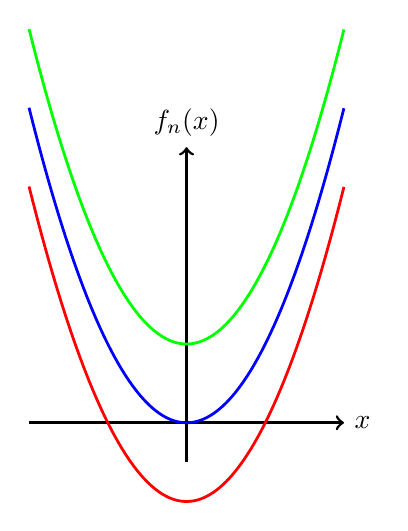
\begin{tikzpicture}
            \draw[->,line width=1pt] (-2,0) -- (2,0) node[right]{$x$};
            \draw[->,line width=1pt] (0, -0.5) -- (0, 3.5) node[above]{$f_n(x)$};
            \draw[red, line width=1pt, domain=-2:2, samples=100] plot(\x,{(\x)^2-1});
            \draw[blue, line width=1pt, domain=-2:2, samples=100] plot(\x,{(\x)^2});
            \draw[green, line width=1pt, domain=-2:2, samples=100] plot(\x,{(\x)^2+1});
        \end{tikzpicture}
    \end{figure}
    
\end{example}

ограниченная, но не равностепенно непрерывная
\begin{example}
    $C[0,1], f_n(x) = x^n$. $\seq{f_n}$ -- ограничены, но не равностепенно непрерывны.
\end{example}


\begin{theoremwobox}[достаточные условия равностепенной непрерывности]
    $(K, \rho)$ -- компакт, $\Phi \subset C(K)$.
    Сначала какие-то абстрактные множества, потом будут более конкретные.
    \begin{enumerate}
        \item Если $\exists M > 0, \alpha > 0, \beta > 0$ такие что 
        \item \begin{multline*}
            \forall f \in \Phi, (\forall x,y \in K \rho(x,y) < \beta) \Rightarrow |f(x) - f(y)| \leq M(\rho(x,y))^\alpha \\
            \Rightarrow \Phi \in (EC)
        \end{multline*}
        \item $C[a,b], \Phi \subset C[a,b]$, пусть $\exists L > 0$ 
        \[ \forall f \in \Phi \, \exists f^\prime(x), x \in (a,b), |f^\prime(x)| \leq L \Rightarrow \Phi \in (EC) \]
        \item чуть более общий случай. $K \subset G \subset \bR^n$, $K$ -- компакт, $G$ -- открытое.
        \[ \exists L > 0 : \forall f \in \Phi, \exists \left| \frac{\partial f}{\partial x_j}  (x) \right| (1 \leq j \leq n), \forall f \in G \,  \Rightarrow \Phi \in (EC)  \] 
        \item про аналитические функции. предполагать можно будет гораздо меньшее. 
        $K \subset G \subset \bC$, $G$ -- открытое, $K$ -- компакт. 
        \[ \exists L > 0, f \in \Phi, f \text{ аналаитическая в } G, \exists f^\prime(x), \underbrace{|f(x)|}_{\text{ТУТ}} \leq L, \forall x \in G \] 
    \end{enumerate}
        ТУТ НЕ ПРОИЗВОДНАЯ, НА ЭКЗАМЕНЕ ЧАСТО ОШИБАЮТСЯ!!!!
\end{theoremwobox}

Аналитичность -- фантастическое свойство, в отличие от, например, дифференцируемости. Именно из-за неё ТАМ как раз и не производная.

\begin{proof}[1]
    Пусть $\varepsilon > 0$, $x, y \in K$, пусть $\rho(x,y) < \beta$, пусть $\delta < \beta, \rho(x,y) < \delta, \delta(\varepsilon) = ?$. 
    \begin{gather*}
        f \in \Phi \Rightarrow |f(x) - f(y)| \leq M \rho(x,y)^\alpha < M \delta^\alpha \leq \varepsilon \\
        \Rightarrow \delta \leq \left( \frac{\varepsilon}{M} \right)^{\frac{1}{\alpha}}, \\
        \delta(\varepsilon) = \min \{ \beta, \left( \frac{\varepsilon}{M} \right)^{\frac{1}{\alpha}} \},
    \end{gather*}
\end{proof}

Будем сводить остальные доказательства к первому пункту, находя $M, \alpha, \beta$. Второй пункт теперь совсем лёгкий. 
\begin{proof}[2]
    $\Phi \subset C[a,b], \, x,y \in [a,b], f \in \Phi$. Для оценки разности $f(x) - f(y)$ воспользуемся теоремой Лагранжа. 
    \begin{multline*}
        f(x) - f(y) = f^\prime(c)(x-y) \Rightarrow |f(x) - f(y)| \leq |f(c)||x-y| \leq L|x-y| \\
        M = L, \alpha = 1, (\beta - \forall) \stackrel{1}{\Rightarrow} \Phi \in (EC)
    \end{multline*}
\end{proof}

\begin{proof}[3]
    Пусть $z, y \in K$ такие что $[z,y] \subset G, f \in \Phi$ 
Оценим разность $f(y) - f(z)$. 
    \begin{gather*}
        \Gamma: [0,1] \rightarrow [y,z] \\
        \Gamma(t) = ty + (1-t)z, \Gamma(0) = z, \Gamma(1) = y \\
        \text{ опять можем воспользоваться теоремой Лагранжа } \\
        f(y) - f(z) = f(\Gamma(1)) - f(\Gamma(0)) = (f(\Gamma(c)))^\prime_t \\
        (f(\Gamma(t)))^\prime_t = (f(ty + (1-t)z))^\prime_t = \sum^n_{j=1} \frac{\partial f}{\partial x_j} (\ldots) (y_j - z_j) \\
        |f(\Gamma(t))^\prime| \leq L \sum^n_{j=1} |y_j - z_j| \stackrel{\text{КБШ}}{\leq} \sqrt{n} \left( \sum^n_{j=1} (y_j - z_j)^2 \right)^\frac{1}{2} = L \sqrt{n} \rho(y,z)
    \end{gather*}
    Если выбртаь $\beta$ достаточно маленьким, то наш отрезок будет лежать в этом компакте. $F = \bR^n \setminus G$ -- замккнутое, $\rho(x,F)$ -- непрерывная функция  в 
    $\bR^n$ $\Rightarrow \rho(x,F)$ непрерывна на $K \Rightarrow \, \exists x_o \in K, \rho(x_0,F) = \min_{x \in K} \rho(x,F)$

    \begin{gather*}
        x_0 \notin F \Rightarrow \rho(x_0, F) > 0, r := \rho(x_0, F) \\
        \forall x \in K \, B_r(x) \subset G, \beta = r \\
        \rho(x,y) < r \Rightarrow y \in B_r(x) \subset G \Rightarrow \\
        \text{ отрезок } [x,y] B_r(x) \subset G \\
        \Rightarrow |f(x) - f(y)| \leq L \sqrt{n} \rho(x,y)
    \end{gather*}
    $z$ и $y$, которые с самого начала были выбраны вместо $x$ и $y$, чтобы не смущаться от $dx$, обратно превратились в $x$ и $y$, все же поняли? \\
    На пальцах: наш компакт настолько утоплен в $G$, что если мы возьмём шарик радиуса $r$, то шарик всё еще лежит в $G$.
\end{proof}

\begin{proof}[4]
    Букву $r$, которую мы нашли в предыдущем пункте, будем изо всех сил использовать. $K \subset G \subset \bC$. В 3 пункте выяснили, что 
    $\exists r > 0: B_r(x) \subset G \, \forall x \in K, \beta = \frac{r}{3}$.
    \begin{gather*}
        x,y \in K, \rho(x,y) < \beta, \gamma = \{ \zeta \in \bC: |x - \zeta| = 2 \beta \} \\
        f \in \Phi
        \intertext{  разницу собираемся оценивать с помощью формулу Коши, поэтому никакие проивзодные и не нужны!!!} \\
        f(x) = \frac{1}{2 \pi i} \int_\gamma \frac{f(\zeta)}{\zeta - x} d \zeta \\
        f(y) = \frac{1}{2\pi i} \int_\gamma \frac{f(\zeta)}{\zeta - y} d\zeta \\
        f(x) - f(y) = \frac{1}{2 \pi i} \int_\gamma f(\zeta) \frac{x-y}{(\zeta-x)(\zeta - y)} d \zeta \\
        \intertext{оцениваем самым грубом образом, отправляя модули под интегралы} \\
        |f(\zeta)| \leq L, |\zeta - x| = 2 \beta, |z-y| \geq \beta 
    \end{gather*}
    \begin{multline*}
        |f(x) - f(y)| \leq \frac{1}{2 \pi} L \cdot |x-y| \cdot |\gamma| \cdot \frac{1}{(2\beta) \cdot \beta} = |x-y|L \frac{(2\beta) \cdot 2 \pi}{(2 \pi)(2 \beta) \beta} = \\
        = \frac{L}{\beta} |x-y|
    \end{multline*}
    и в обозначениях 1 пункта получаем $M = \frac{L}{\beta}, \alpha = 1, \beta = \frac{r}{3}, \stackrel{(1)}{\Rightarrow} \Phi \in (EC)$
\end{proof}
Перед тем, как мы покинем относительно компакты, пара упражнений, которые на экзамене спрашивали в качестве задачи на 5.
\begin{statement}
    $1 \leq p < + \infty$. $\Phi \subset l^p, \Phi$ -- относительно компактно $\Leftrightarrow$ 
    \begin{enumerate}
        \item $\Phi$ -- ограничено в $l^p$ \\
        \item $\forall \varepsilon > 0 \, \exists N \in \bN : \forall x = \seq{x_j}^\infty_{j=1} \in \Phi, \left( \sum^\infty_{j=N+1} |x_j|^p \right)^{\frac{1}{p}} < \varepsilon$ 
    \end{enumerate}
\end{statement}
\begin{statement}
    $\Phi \subset C_0, \Phi$  -- относительно компактно $\Leftrightarrow$ 
    \begin{enumerate}
        \item $\Phi$ -- ограничено \\
        \item $\varepsilon > 0 \, \exists N \in \bN : \forall x \in \Phi \quad \sup_{j \geq N+1} |x_j| < \varepsilon $
    \end{enumerate}
\end{statement}
Мы сейчас находимся на перепутье функционального анализа. Можно отправиться в Гильбертовы пространства, в линейные операторы или еще куда-то. Изучить-то придётся всё, но
мы начинаем линейные операторы. 
\end{document}
